\section{Auswertung} \label{sec:Auswertung}

In \autoref{tab:messwerte} sind sämtliche zur Verfügung gestellten Messwerte aufgelistet.
Der (gerundete) Fehler der Zählrate $Z$, der sich aus $\sqrt{N}$ berechnet, wurde ebenfalls angegeben.
Die Ablesegenauigkeit des Amperemeters ist konstant $\symup{\Delta}I=\SI{0.05}{\micro\ampere}$.

\begin{table}[H]
  \centering
  \caption{Übersicht aller aufgenommenen Messwerte.}
  \label{tab:messwerte}
  \begin{tabular}{c c c}
  \toprule
  $U \mathbin{/} \si{\volt}$ &
  $N \mathbin{/} \si{{Imp} \per 60 \second}$ &
  $I \mathbin{/} \si{\micro\ampere}$ \\
  \midrule
  \expandableinput{build/table_messwerte.tex}
  \bottomrule
  \end{tabular}
\end{table}


\subsection{Aufnahme der Geiger-Müller-Charakteristik}

% Die Integrationszeit pro Zählrohrspannung betrug t = 60s, damit die Zählrate
% im Geiger-Plateau in der Größenordnung von N = 10000 Imp liegt. (Warum? Begründung
% nicht vergessen)

\begin{figure}
  \centering
  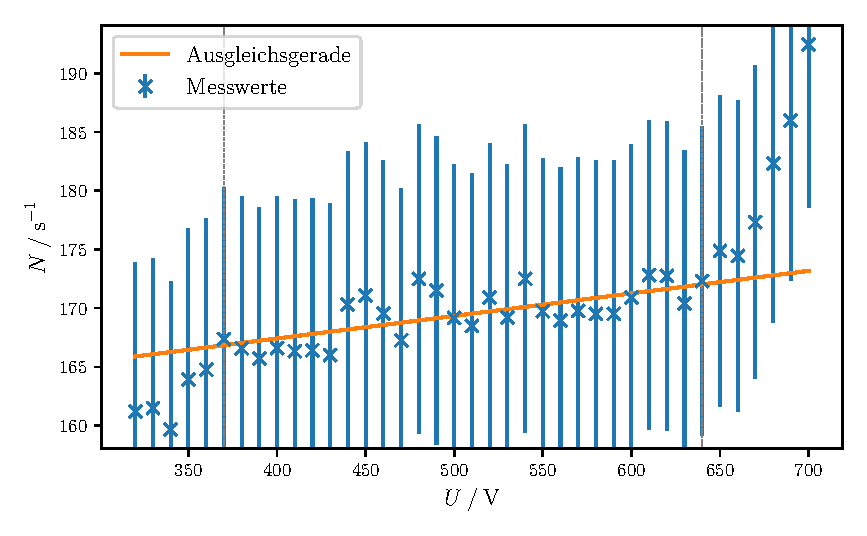
\includegraphics[width=\textwidth]{build/plot1.pdf}
  \caption{Impulsrate in Abhängigkeit der Spannung.}
  \label{fig:plot1}
\end{figure}

Weil die Zählraten Poisson-verteilt sind, sind die Messunsicherheiten durch $\symup{\Delta}N = \sqrt{N}$ gegeben.
Das Plateau liegt in etwa zwischen $\SI{370}{\volt}$ und $\SI{640}{\volt}$
und ist in \autoref{fig:plot1} durch gestrichelte Linien begrenzt.
% /gekennzeichnet
Die Plateaulänge beträgt also ungefähr $\SI{270}{\volt}$.
Für diesen Bereich wurde
der Plateauanstieg durch
eine Regressionsgerade
zu $\SI{19.198(3727)}{{Imp}\per\second\per\kilo\volt}$
% und Achsenabschnitt
bestimmt.

\subsection{Bestimmung der Totzeit}

\subsubsection{Zwei-Quellen-Methode}
\label{sec:totzeit_zweiquellen}

Bei einer Messzeit von $t = \SI{120}{s}$ wurden folgende Zählraten gemessen:

\begin{align*}
N_{1}   &= \SI{96041} {{Imp} \per 120 \second} \\
N_{1+2} &= \SI{158479}{{Imp} \per 120 \second} \\
N_{2}   &= \SI{76518} {{Imp} \per 120 \second} \\
\end{align*}

Nach \autoref{eqn:totzeit} ergibt sich daraus eine Totzeit von $T \approx \SI{115(4)}{\micro\second}$.
Die Messunsicherheit
% welche auch nach der Gaußschen Fehlerfortpflanzung bestimmbar wäre,
wurde mit dem Python-Paket \textit{uncertainties} berechnet.

% Der Fehler kann gemäß der Gaußschen Fehlerfortpflanzung folgendermaßen berechnet werden:
% \begin{equation*}
%   \symup{\Delta}T =
%   \frac{N_{1+2}-N_2}{2N_1^2N_2} \cdot \symup{\Delta}N_1 +
%   \frac{N_{1+2}-N_1}{2N_2^2N_1} \cdot \symup{\Delta}N_2 -
%   \frac{1}{2N_1N_2} \cdot \symup{\Delta}N_{1+2}
% \end{equation*}


\subsubsection{Oszilloskop}
\label{sec:totzeit_oszilloskop}

Die Zeitachse am Oszilloskop bemisst sich auf $\SI{100}{\micro\second \per {DIV}}$,
sodass jeder Strich $\SI{20}{\micro\second \per {DIV}}$ entspricht.

Es wurde nun die Totzeit als Zeit zwischen dem ersten und zweiten Puls abgelesen,
wie in \autoref{fig:totzeit_oszilloskop} dargestellt ist.
Diese ergab sich zu $T \approx \SI{110(20)}{\micro\second}$,
wobei die Unsicherheit als der Abstand zwischen zwei Strichen abgeschätzt ist.

\begin{figure}[H]
  \centering
  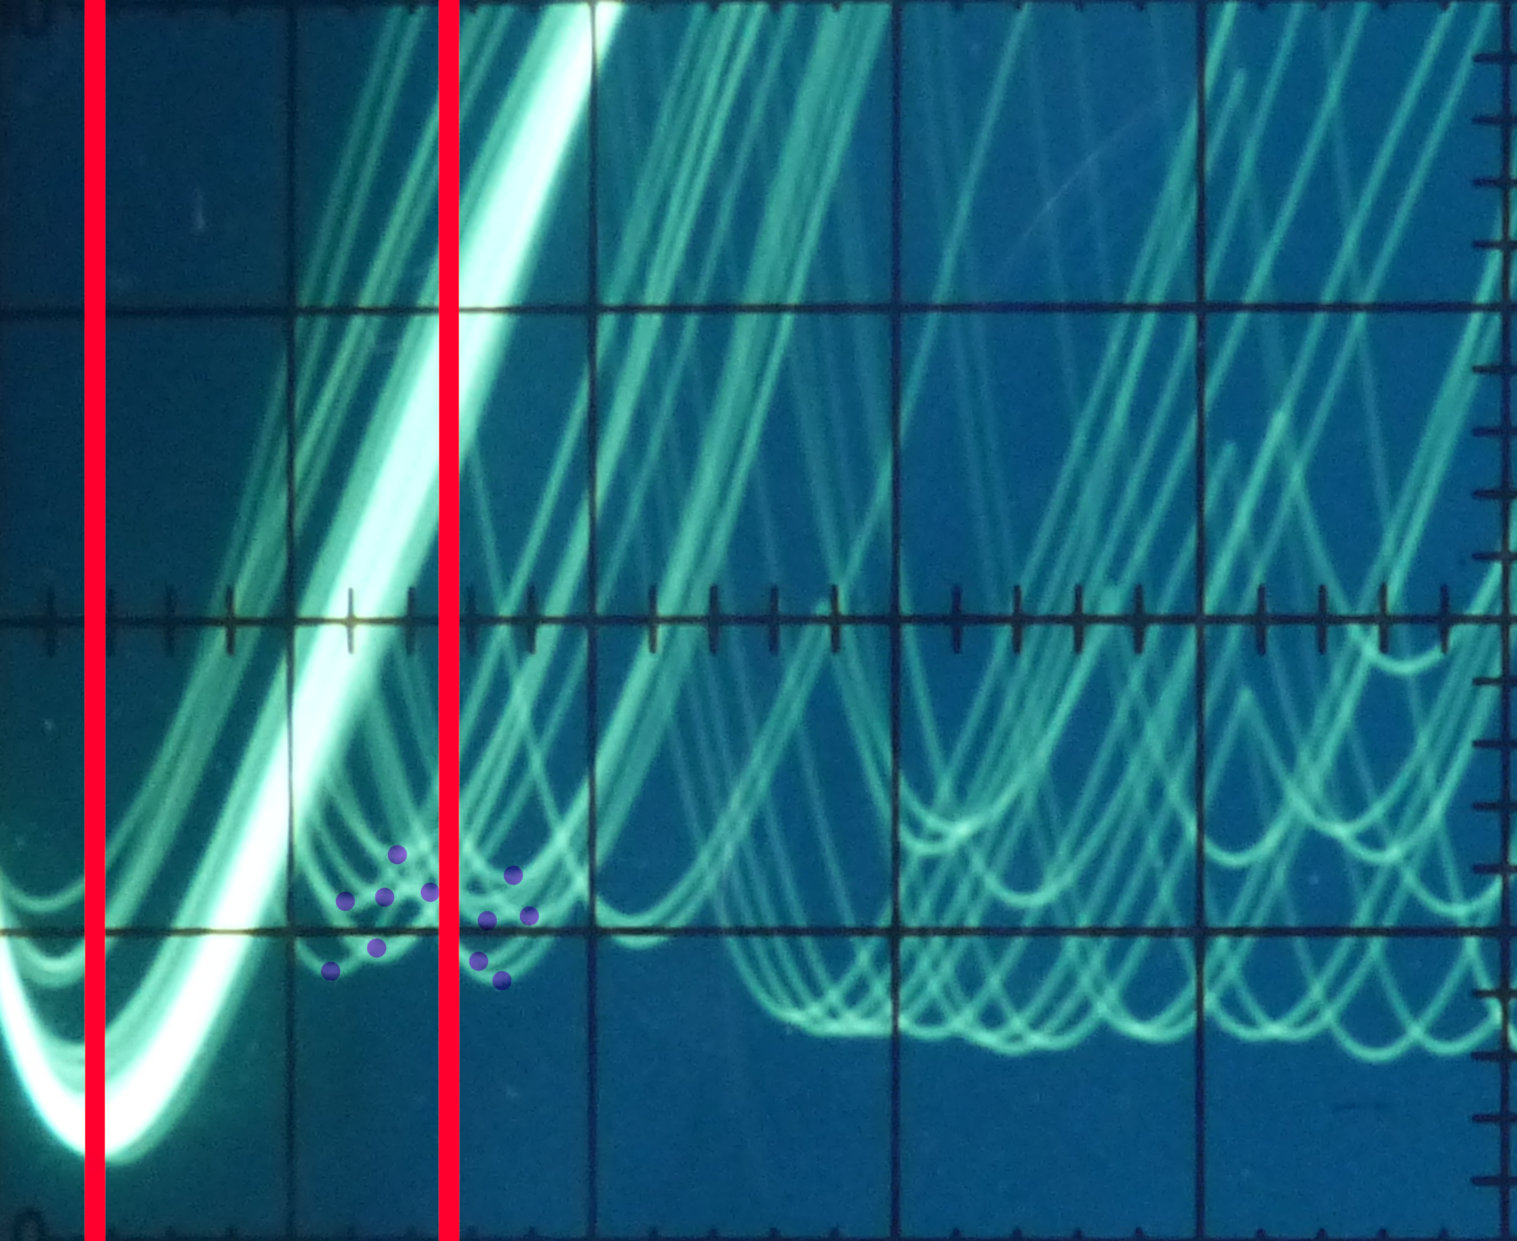
\includegraphics[width=0.75\textwidth]{content/img/totzeit_oszilloskop.jpg}
  \caption{Momentaufnahme des Oszilloskops mit eingezeichneten Extrema und Zeiten \cite{oszilloskop}.}
  \label{fig:totzeit_oszilloskop}
\end{figure}

% In DatenHinweiseGeigerMueller.pdf steht: Bestimmung des Zählrohrstroms 🤔
\subsection{Bestimmung der pro Teilchen freigesetzten Ladungen}

Gemäß \autoref{eqn:Teilchenzahl} lässt sich aus der Anzahl eingefallener Teilchen und dem Zählerstrom
auf die Anzahl der freigesetzten Ladungen pro einfallendem Teilchen schließen.
In \autoref{fig:plot2} ist dieses Verhältnis gegen die anliegende Spannung aufgetragen.
Die Messunsicherheit wurde wieder mit \textit{uncertainties} berechnet.

Im Mittel ergibt sich $Z=\num{3.43(6)e+10}$.

\begin{table}[H]
  \sisetup{separate-uncertainty=true}
  \centering
  \caption{Zahl der pro einfallendem Teilchen freigesetzten Ladungen.}
  % \label{tab:messwerte}
  \begin{tabular}{c c c c}
  \toprule
  $U \mathbin{/} \si{\volt}$ &
  $N \mathbin{/} \si{{Imp} \per 120 \second}$ &
  $I \mathbin{/} \si{\micro\ampere}$ &
  $Z [10^{10}]$ \\
  \midrule
  \expandableinput{build/table_zaehlrohrstrom.tex}
  \bottomrule
  \end{tabular}
\end{table}

\begin{figure}[H]
  \centering
  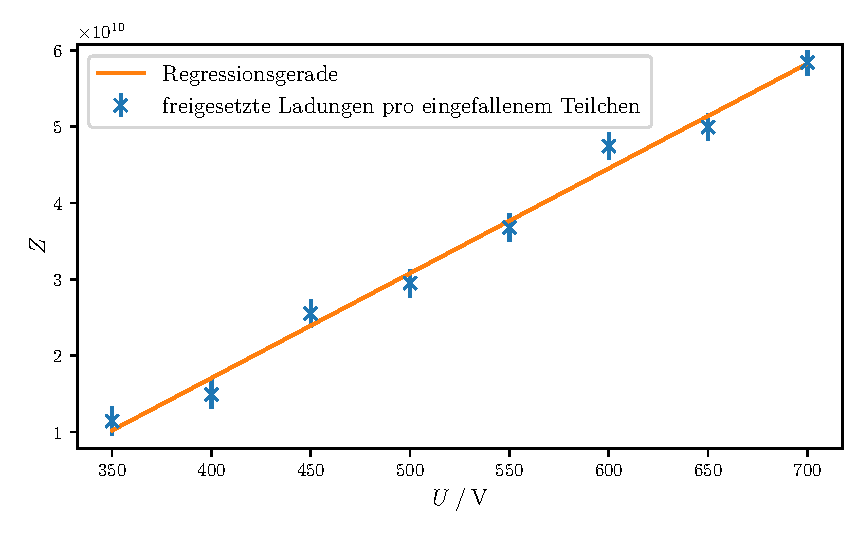
\includegraphics[width=\textwidth]{build/plot2.pdf}
  \caption{Zahl der freigesetzten Ladungen pro eingefallenem Teilchen in Abhängigkeit der Spannung.}
  \label{fig:plot2}
\end{figure}
